%!TEX root = apostila.tex
\section{SCADA}

SCADA -- \emph{Supervisory Control And Data Acquisition}, são os sistemas do nível 2 da pirâmide de automação. Eles são a interface com os operadores com os sistemas de controle do nível 1. Suas funções são:

\begin{description}
\item[Supervisão], mostrando de forma prática o estado do processo.
\item[Operação], substituindo os painéis de controle. Permite ligar e desligar os equipamentos, definir setpoints, etc.
\item[Controle] de operações simples e que não tenham restrições temporais grandes.
\end{description}

Hoje em dia os sistemas SCADA também tem grande integração com os sistemas acima da pirâmide, e são responsáveis por fornecer dados a estes sistemas e receber informações adicionais, tais como setpoints pré-fixados e receitas. Basicamente o SCADA serve como interface principal dos usuários com os sistemas de automação.

Tipicamente, um sistema SCADA possui:
\begin{description}
	\item[Sinóticos] - Telas representativas do processo.
	\item[Alarmes] - Seja definidos no próprio SCADA seja definidos num elemento de controle (que é o mais comum).
	\item[Gráficos de tendência] - Mostram a variação de variáveis do processo ao longo do tempo.
	\item[Gerador de relatórios] - tipicamente contendo os alarmes e eventos de um determinado período e vários gráficos de tendência. Podem ser gerados devido a uma condição de alarme.
\end{description}

\section{Variáveis}
O sistema SCADA trabalha com informações advindas do nível 1 da pirâmide de automação (CLPs, SDCDs), do nível 3 (PIMS e MES) ou geradas no próprio SCADA. Estas informações são armazenadas em variáveis na base de dados do SCADA, também chamadas de TAGs. Esta variáveis tem associadas a elas um conjunto de informações, dos quais os mais comuns são:

\begin{description}
	\item[Tag] O nome \emph{oficial} da variável. Único para cada uma delas.
	\item[Endereço] A origem da variável --- que memória de qual CLP, etc.
	\item[Descrição] Uma descrição sucinta da variável.
	\item[Valor] Último valor medido.
	\item[Time Stamp] Data e hora em que foi medido o último valor.
\end{description}

São variáveis típicas:
\begin{description}
	\item[Variáveis Analógicas] Tipicamente obtidas dos CLPs em formato bruto e convertidas para valores de engenharia no SCADA. Muitas vezes são também submetidas a um filtro digital no próprio SCADA, para diminuir ruídos.

	É comum que se adicionem limites a uma variável deste tipo relacionados a alarmes da mesma, tais como:
	\begin{itemize}
		\item Lim inferior: valor em UE ser atribuído ao valor 0\% da variável.
		\item Lim superior: valor em UE a ser atribuído ao valor 100\% da variável.
		\item Limite HH: valor em UE para alarme Muito Alto.
		\item Limite H: valor em UE para alarme Alto.
		\item Limite L: valor em UE para alarme Baixo.
		\item Limite LL: valor em UE para alarme Muito Baixo.
	\end{itemize}

	\item[Variáveis Discretas] Tipicamente valores binários.

	Em geral são associadas uma descrição dos estados 0 e 1, tais como: aberto/fechado, desligado/ligado, parado/funcionando, e assim por diante.
	\item[Totalizadores] Pode ser um contador de pulsos ou um integrador de um valor analógico (de vazão, por exemplo). Em alguns casos o valor totalizado é calculado no CLP e em outros no próprio SCADA.

	Um totalizador pode ser referente a um período (hora, turno, dia, mês, ano), a um equipamento, a um operador, a um produto ou a alguma outra informação.

	\item[Controladores PID] Um controle do tipo PID (Proporcional, Integral e Derivativo) é muito usado para garantir que uma determinada grandeza observada (variável de processo) acompanhe o valor desejado (setpoint) pelo ajuste contínuo de uma grandeza controlada (variável manipulada). CLPs mais modernos já contam com algoritmos de controle PID que dependem das constantes definidas no controlador (setpoint, Kp, Ki e Kd).

	No sistema SCADA, uma variável do tipo PID armazena os valores destas constantes, que podem então ser ajustados pelo operador ou por um algoritmo de ajuste. Tipicamente o CLP e o SCADA definem formas de sobrepassar o controlador PID permitindo o controle da variável maipulada diretamente pelo operador.
	\item[Equipamentos] Corresponde a um equipamento de processo qualquer: motor, transportador de correia, bomba, reator, etc. Conta com valores discretos que informam o status do equipamento, bem como com um horímetro, que fornece o total de horas de operação do equipamento.

	Normalmente permite sobrepassar o controle automático do equipamento e realizar ações de comando, tais como ligar e desligar.
\end{description}

\section{Sinótico}
Boa parte do uso de um sistema SCADA é como uma IHM -- Inteface Homem Máquina. Neste ponto ele substitui os painéis ou quadros sinóticos (vide figura \ref{fig:painel_sinotico}), usados ainda em algumas aplicações simples mas muito usados antigamente.


\begin{figure}[hb]
	\centering
	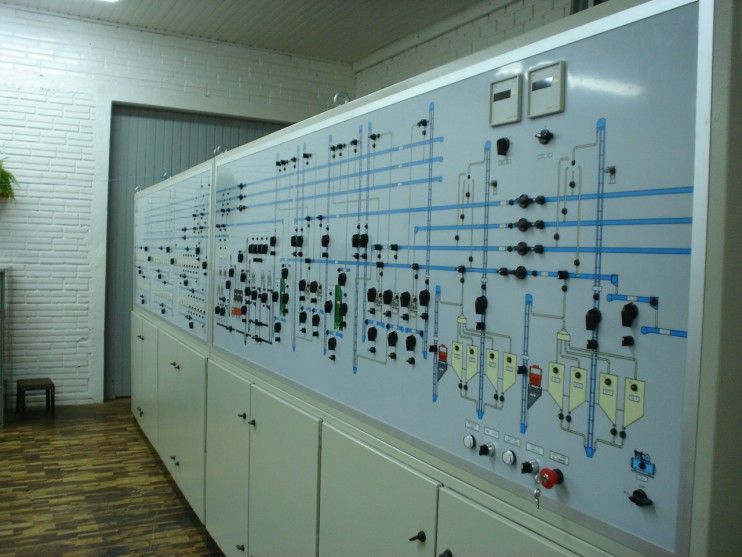
\includegraphics[width=0.6\textwidth]{figuras/painel_sinotico}
	\caption{Exemplo de um antigo painel sinótico.}\label{fig:painel_sinotico}
\end{figure}
Um sinótico é uma representação gráfica simplificada de um sistema -- uma síntese ótica. Num sistema SCADA, um sinótico representa uma área do processo em um certo nível de detalhe.

Tipicamente se tem um sinótico geral para uma planta, do qual se podem abrir sinóticos específicos de uma determinada área (numa hierarquia de sinóticos) ou a uma visão de uma outra camada do mesmo sinótico (por exemplo, um mostrando características elétricas e outro características termodinâmicas de um processo).

\begin{figure}[hb]
  \centering
  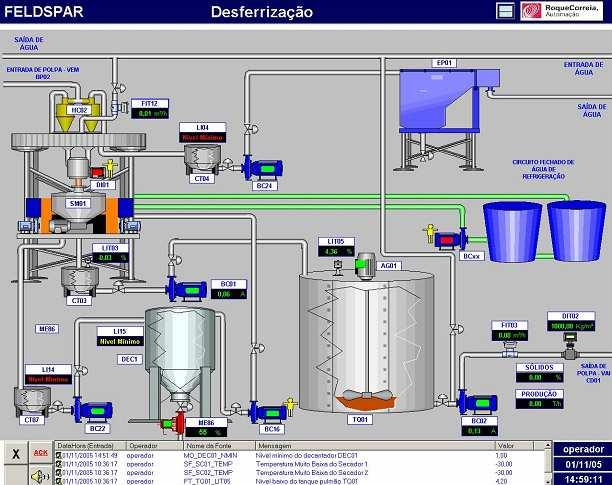
\includegraphics[width=0.6\textwidth]{figuras/sinotico_feldspar}
  \caption{Exemplo de um sinótico em um SCADA.}\label{fig:sinotico_feldspar}
\end{figure}


\subsection{Requisitos}
\label{sub:Requisitos}

O projeto de um sinótico é bastante complexo e foge um tanto das competências típicas de um engenheiro. Ao projetar uma IHM o projetista deve trabalhar com vários requisitos ergonômicos e de comportamento humano, procurando:

\begin{itemize}
	\item Diminuir a chance de erro do operador, principalmente nos
	momentos de maior demanda operacional, coincidentes com o aumento
	do stress.
	\item Evitar as situações de monotonia que levam à desconcentração do
	operador. Sinóticos pouco representativos do processo e sem atrações
	de animação ou com muitos dados tabulares levem ao desinteresse.
	\item Evitar situações que acarretam cansaço.
	\item Manter o operador sempre atento ao que realmente interessa. Sinóticos muito cheios trazem
	excesso de informações que o operador não é capaz de processar. Os
	alarmes e informações devem ser mostrados apenas em casos de exceção para evitar avalanches de alarmes.
	\item Evitar consulta a referências externas ao sistema. Se necessário, o operador deve poder	tirar dúvidas quanto a operação do sistema no próprio SCADA.

\end{itemize}

Estudos ergonômicos voltados para a atenção de pessoas a IHMs mostram que os olhos tendem a se focar primeiro em uma imagem grande ao invés de uma pequena, em cores mais saturadas (brilhantes), em formas simétricas ao invés de formas assimétricas e em algo que se move e pisca em contraponto a uma imagem estática. Estes conhecimentos devem ser utilizados para a construção do sinóptico bem balanceado.


São bons costumes em um sinótico:
\begin{itemize}
	\item Utilizar representação gráfica dinâmica (animações) para evitar a monotonia, mas.
	\item Evitar objetos grandes piscantes, que cansam e distraem.
	\item Representar equipamentos por desenhos de acordo com sua forma e
	tamanhos reais, porém a representação fotográfica com excesso de
	detalhes, sombra, etc. é desaconselhável.
	\item Deixar o mais óbvio e intuitivo possível a seqüência para ligar ou desligar equipamentos ou realizar ações
	de controle similares. Deve-se utilizar de metáforas visuais com equipamentos físicos.
	\item Utilizar mensagens devem ser claras, explícitas e auto suficientes. Um contra
	%exemplo: ``Erro 46A: Execute o procedimento de emergência 78´´.

\end{itemize}

Um determinado valor pode ser mostrado num sinótico de diversas formas. As mais comuns são:
\begin{description}
	\item[Texto] -- Para uma variável analógica, exibe seu valor em unidades de engenharia. A cor do texto pode servir
	para codificar o status da variável (por exemplo, se valor muito alto ou muito baixo). Para um variável binária é comum atribuir o significado: ABERTO/FECHADO, LOCAL/REMOTO ou
	LIGADO/DESLIGADO.
	\item[Barras horizontais e verticais] -- Fornecem uma representação percentual do valor da variável. Podem ser utilizados para mostrar o enchimento de um silo, tanque, reator, etc.
	\item[Deslocamento e rotação] --  Podem ser pelo valor de uma variável analógica ou relacionados a valores discretos, tais como sensores de fim de curso, por exemplo.
	\item[Mostradores Circulares] -- Evocam os mostradores de ponteiro de instrumentos indicadores analógicos.
	\item[Tendência] -- Exibe o gráfico dos últimos valores da variável em função do tempo.
	\item[Associação a cor (ou outro atributo) de um objeto] -- A cor do objeto muda de acordo com o status da variável associada.
	\item[Associação a um par de objetos complementares] -- Os dois objetos ocupam fisicamente a mesma posição no sinótico. Quando
	a variável está em 0 o objeto chave aberta, por exemplo, é exibido, quando está em 1 a chave é mostrada na posição fechada.
\end{description}

Deve-se sempre buscar a representação mais natural para cada variável. Por exemplo, enchimento para tanques e silos, rotação para um
forno de cimento ou britador de martelos, etc.


\section{Alarmes e Eventos}
\label{sec:Alarmes e Eventos}
Outra função do SCADA é mostrar e armazenar todos os eventos significativos que ocorreram no processo, que são classificados em simples eventos a serem registrados (por exemplo: troca de operador, fim de fabricação de lote, etc) e alarmes, que são situações indesejadas e que requerem ações corretivas.

Os alarmes são classificados por prioridade, definida por dois fatores: severidade das consequências e tempo requerido para tomar ações corretivas. Tipicamente os sistemas SCADA usam uma classificação numérica para a prioridade dos alarmes, mas uma classificação mais intuitiva é a de prioridade baixa, média, alta e crítica. Tome-se por exemplo o sinal de temperatura de um forno. Para um determinado processo, pode-se considerar que:
\begin{itemize}
	\item Uma temperatura baixa (L) durante a operação do forno indica um problema no controle, mas que a princípio não causará dano imediato. Atribui-se um alarme de baixa prioridade a este evento.
	\item Uma temperatura muito baixa (LL) indica que o processo já não mais funcionará e talvez vá se perder aquele lote. Atribui-se um alarme de prioridade média.
	\item Uma temperatura alta (H) já indica perda de material e pode levar a problemas piores se não for corrigido rápido. Atribui-se um alarme de alta prioridade.
	\item Uma temperatura muito alta (HH) já é um risco iminente de incêndio. Atribui-se um alarme de prioridade crítica.
\end{itemize}

Estes alarmes e eventos podem ser definidos no próprio SCADA ou no CLP, enviados ao SCADA como uma variável booleana.

Um alarme deve ser mostrado no painel de controle do SCADA para chamar atenção do operador. A partir do momento que um alarme ocorre, ele precisa ser normalizado (a situação que o gerou deve ser corrigida, seja por atuação do operador ou pelo controle automático do processo) e o operador precisa marcar no supervisório que identificou o alarme (chama-se reconhecer o alarme). A ideia por trás disso é que uma vez que o operador reconheceu o alarme, o supervisório não mais precisa ficar chamando a atenção do operador para aquele problema.

Com base nisto, pode-se apresentar o alarme na tela da seguinte forma (entre outras possibilidades):
\begin{description}
	\item[\textcolor{red}{Vermelho Piscante}] Alarme não reconhecido.
	\item[\textcolor{red}{Vermelho}] Alarme já reconhecido.
	\item[\textcolor{yellow}{Amarelo}] Normalizado e não reconhecido.
	\item[\textcolor{green}{Verde}] Normalizado e reconhecido.
\end{description}

Os alarmes e eventos são armazenados em uma base de dados com os seguintes dados:
\begin{itemize}
	\item Alarme ou evento disparado
	\item Valor no momento do alarme
	\item Descrição do evento
	\item Data e hora do evento
\end{itemize}

A normalização ou reconhecimento de um alarme conta como eventos que também são armazenados nesta base de dados.

Esta base de dados pode ser consultada no próprio SCADA, pode ser inserida num relatório automático e/ou enviada para sistemas acima na pirâmide automação.

\section{Arquitetura de Hardware e Software}
\label{sec:Arquitetura de Hardware e Software}

Sistemas SCADA modernos dependem bastante da estrutura da rede de computadores. Estes sistemas permitem dividir as tarefas do SCADA em vários computadores: Um servidor de entrada e saída, para comunicação com os CLPs, um servidor de banco de dados, para armazenar e distribuir os dados obtidos, um gerenciador de alarmes e várias estações de acesso, que permitem acessar o sistema de vários pontos.  Cada um destes sistemas pode, além disto, ter uma redundância, de modo que se um computador falhar outro assume na mesma hora, sem perda de funcionalidade. Ao mesmo tempo, para sistemas simples ainda é possível ter todas estas funções rodando em um único computador.

Cada vez mais comum é ter um servidor web, que permite disponibilizar toda a ferramenta SCADA num navegador de internet. Para tanto deve-se ter um cuidado com o acesso a esta rede, o que normalmente é feito através de VPNs - \emph{Virtual Private Networks}, que criam uma rede privada virtual sobre a internet usando criptografia para prevenir acessos indesejados.
